\documentclass{article}\usepackage[]{graphicx}\usepackage[]{color}
%% maxwidth is the original width if it is less than linewidth
%% otherwise use linewidth (to make sure the graphics do not exceed the margin)
\makeatletter
\def\maxwidth{ %
  \ifdim\Gin@nat@width>\linewidth
    \linewidth
  \else
    \Gin@nat@width
  \fi
}
\makeatother

\definecolor{fgcolor}{rgb}{0.345, 0.345, 0.345}
\newcommand{\hlnum}[1]{\textcolor[rgb]{0.686,0.059,0.569}{#1}}%
\newcommand{\hlstr}[1]{\textcolor[rgb]{0.192,0.494,0.8}{#1}}%
\newcommand{\hlcom}[1]{\textcolor[rgb]{0.678,0.584,0.686}{\textit{#1}}}%
\newcommand{\hlopt}[1]{\textcolor[rgb]{0,0,0}{#1}}%
\newcommand{\hlstd}[1]{\textcolor[rgb]{0.345,0.345,0.345}{#1}}%
\newcommand{\hlkwa}[1]{\textcolor[rgb]{0.161,0.373,0.58}{\textbf{#1}}}%
\newcommand{\hlkwb}[1]{\textcolor[rgb]{0.69,0.353,0.396}{#1}}%
\newcommand{\hlkwc}[1]{\textcolor[rgb]{0.333,0.667,0.333}{#1}}%
\newcommand{\hlkwd}[1]{\textcolor[rgb]{0.737,0.353,0.396}{\textbf{#1}}}%
\let\hlipl\hlkwb

\usepackage{framed}
\makeatletter
\newenvironment{kframe}{%
 \def\at@end@of@kframe{}%
 \ifinner\ifhmode%
  \def\at@end@of@kframe{\end{minipage}}%
  \begin{minipage}{\columnwidth}%
 \fi\fi%
 \def\FrameCommand##1{\hskip\@totalleftmargin \hskip-\fboxsep
 \colorbox{shadecolor}{##1}\hskip-\fboxsep
     % There is no \\@totalrightmargin, so:
     \hskip-\linewidth \hskip-\@totalleftmargin \hskip\columnwidth}%
 \MakeFramed {\advance\hsize-\width
   \@totalleftmargin\z@ \linewidth\hsize
   \@setminipage}}%
 {\par\unskip\endMakeFramed%
 \at@end@of@kframe}
\makeatother

\definecolor{shadecolor}{rgb}{.97, .97, .97}
\definecolor{messagecolor}{rgb}{0, 0, 0}
\definecolor{warningcolor}{rgb}{1, 0, 1}
\definecolor{errorcolor}{rgb}{1, 0, 0}
\newenvironment{knitrout}{}{} % an empty environment to be redefined in TeX

\usepackage{alltt}
\usepackage{graphicx}
\IfFileExists{upquote.sty}{\usepackage{upquote}}{}
\begin{document}



\section*{Problem 1}

\begin{knitrout}
\definecolor{shadecolor}{rgb}{0.969, 0.969, 0.969}\color{fgcolor}
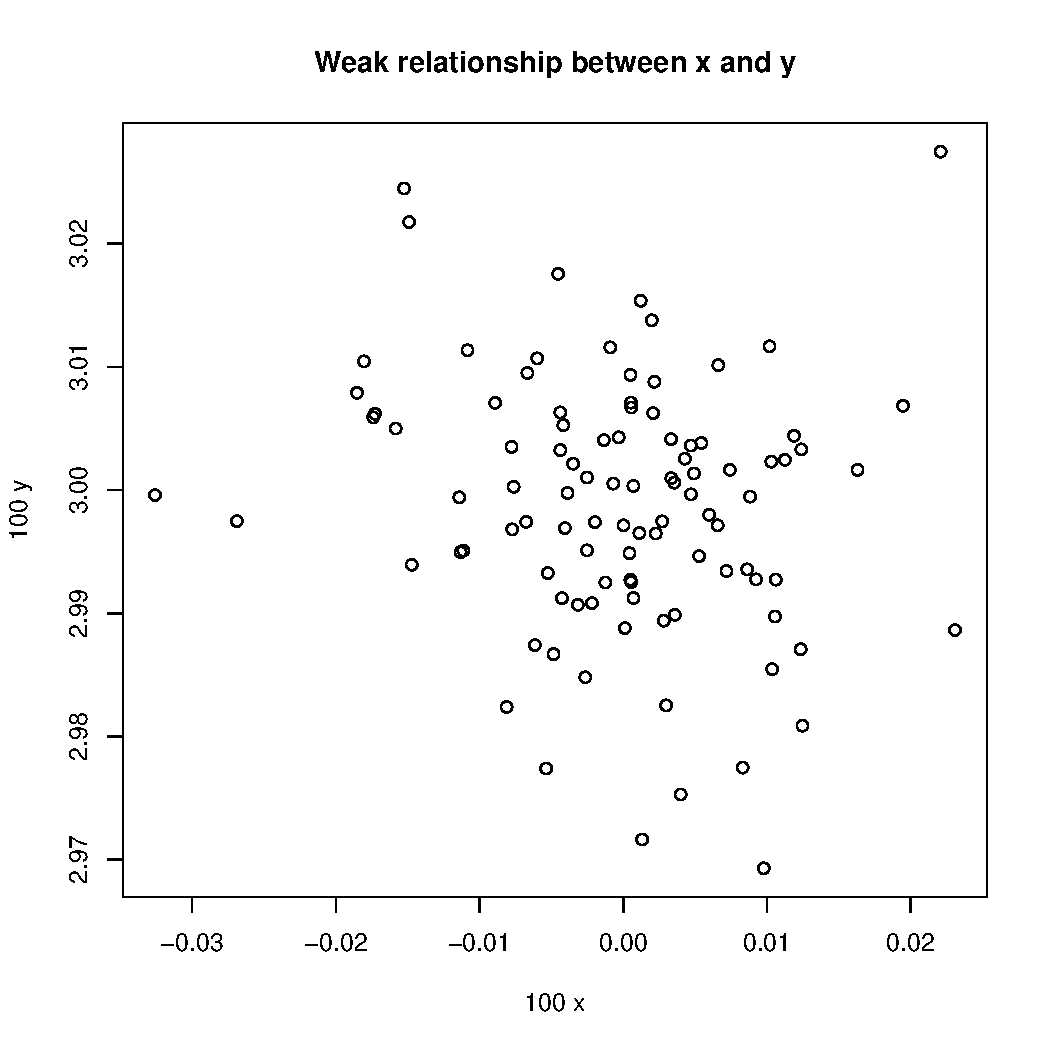
\includegraphics[width=5.5in]{figure/p1-1} 

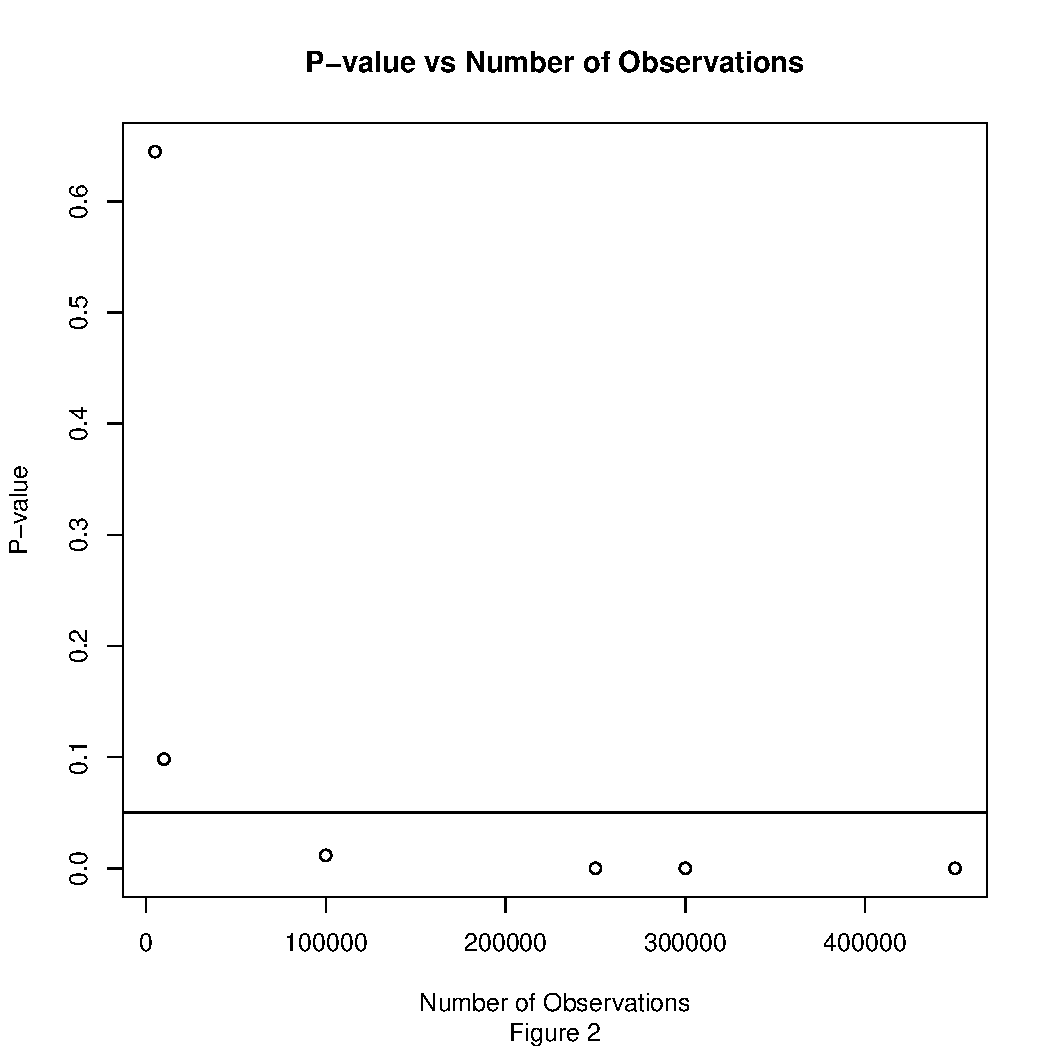
\includegraphics[width=5.5in]{figure/p1-2} 

\end{knitrout}

\noindent We set the parameters to $y = 3 + 0.01*x + e$, for which y has a weak relationship with x.  The correlation is 0.009. We then ran regressions on samples of increasing size, from 10000 to NA and plotted the p-values for each regression.  As seen in the figure, the relationship is consistently statistically significant after 1000000 samples, which shows that as sample size increases, even weak relationships will be shown as significant.


\section*{Problem 2}


\noindent We completed Problem 2b prior to 2a, which is why the code is nearly identical. The correlation between x1 and y is -0.252, while the coefficient in the regression is 0.191, showing that the lurking variable x2 changes the sign.\\



\noindent We chose to comment on the Harvard Circut Court decision on admission of Asian American applicants.  Here, x1 is binomially distributed to mark if the candidate is Asian (5.6\% of the U.S. population is Asian).  x2 is the ``personality'' score as described in the brief, which here is lowered if the applicant is Asian. y is binomially distributed for acceptance to Harvard based on the personality score distribution, which is lower for Asian applicants.  

\section*{Problem 3}
\subsection*{Part a}
\begin{figure}[h!]
% 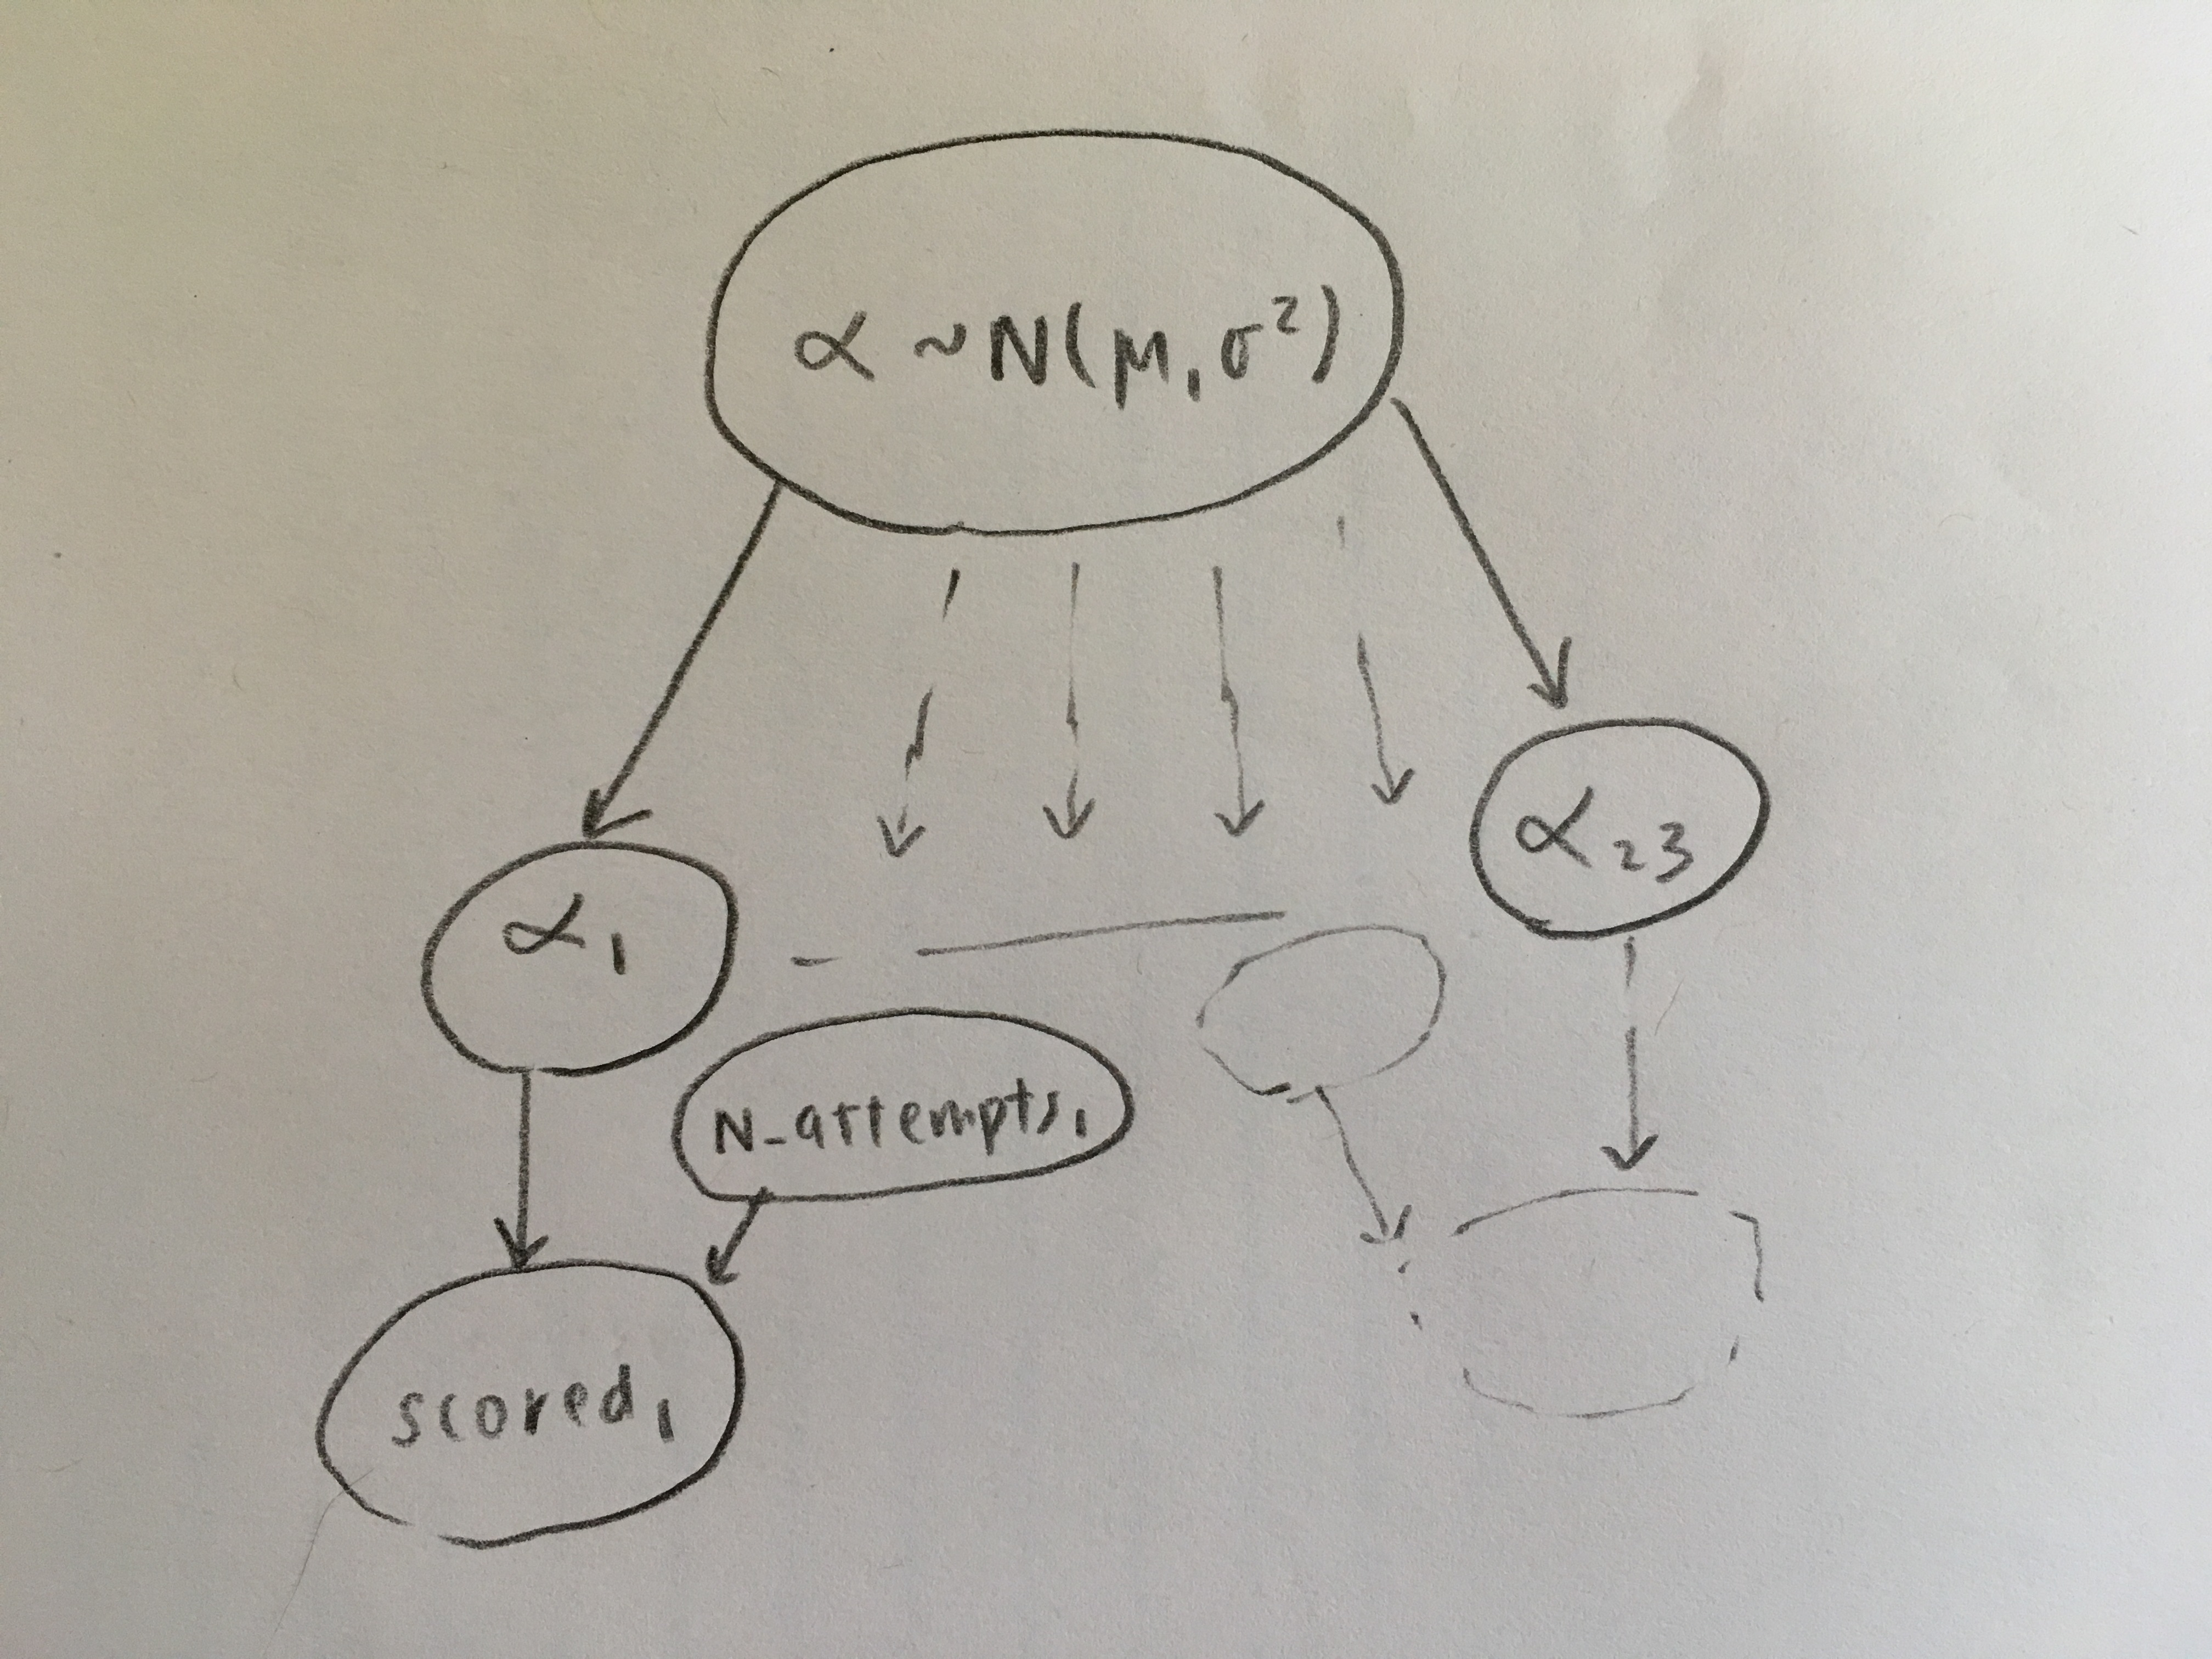
\includegraphics[scale=.1]{/sml310_mp1/p3a.jpg}
\end{figure}

\subsection*{Part b}

% N = game number
% scored[N] = array of scores indexed by game
% attempted[N] = array of number of attemps indexed by game

% mu = overall average skill level
% sigma = overall stdev of skill level, lower bounded by 0

% alpha[N] = array of average skill level indexed by game
% loop samples from ~N(mu, sigma^2)

% alpha_norm ~ N(0, 1)
% scored sum of bernoulli of attempted using prob of alpha(skill level)

\begin{knitrout}
\definecolor{shadecolor}{rgb}{0.969, 0.969, 0.969}\color{fgcolor}\begin{kframe}


{\ttfamily\noindent\bfseries\color{errorcolor}{\#\# Error in compileCode(f, code, language = language, verbose = verbose): Compilation ERROR, function(s)/method(s) not created! /bin/sh: /usr/local/Cellar/gcc/8.2.0/bin/g++-7: No such file or directory\\\#\# make: *** [file1270a3d865789.o] Error 127}}

{\ttfamily\noindent\bfseries\color{errorcolor}{\#\# Error in sink(type = "{}output"{}): invalid connection}}

{\ttfamily\noindent\bfseries\color{errorcolor}{\#\# Error in sampling(object = shaq\_model, data = list(N = nrow(shaq), scored = shaq\$Scored, : object 'shaq\_model' not found}}

{\ttfamily\noindent\bfseries\color{errorcolor}{\#\# Error in extract(shaq\_fit): object 'shaq\_fit' not found}}

{\ttfamily\noindent\bfseries\color{errorcolor}{\#\# Error in hist(samplesPartial\$mu): object 'samplesPartial' not found}}

{\ttfamily\noindent\bfseries\color{errorcolor}{\#\# Error in hist(samplesPartial\$sigma): object 'samplesPartial' not found}}

{\ttfamily\noindent\bfseries\color{errorcolor}{\#\# Error in hist(samplesPartial\$alpha[, 1]): object 'samplesPartial' not found}}

{\ttfamily\noindent\bfseries\color{errorcolor}{\#\# Error in hist(samplesPartial\$alpha[, 2]): object 'samplesPartial' not found}}

{\ttfamily\noindent\bfseries\color{errorcolor}{\#\# Error in mean(samplesPartial\$mu): object 'samplesPartial' not found}}

{\ttfamily\noindent\bfseries\color{errorcolor}{\#\# Error in mean(samplesPartial\$mu): object 'samplesPartial' not found}}

{\ttfamily\noindent\bfseries\color{errorcolor}{\#\# Error in eval(expr, envir, enclos): object 'good' not found}}

{\ttfamily\noindent\bfseries\color{errorcolor}{\#\# Error in eval(expr, envir, enclos): object 'bad' not found}}\end{kframe}
\end{knitrout}

\begin{knitrout}
\definecolor{shadecolor}{rgb}{0.969, 0.969, 0.969}\color{fgcolor}\begin{kframe}


{\ttfamily\noindent\bfseries\color{errorcolor}{\#\# Error in hist(samplesPartial\$mu): object 'samplesPartial' not found}}

{\ttfamily\noindent\bfseries\color{errorcolor}{\#\# Error in hist(samplesPartial\$sigma): object 'samplesPartial' not found}}

{\ttfamily\noindent\bfseries\color{errorcolor}{\#\# Error in hist(samplesPartial\$alpha): object 'samplesPartial' not found}}\end{kframe}
\end{knitrout}



\begin{knitrout}
\definecolor{shadecolor}{rgb}{0.969, 0.969, 0.969}\color{fgcolor}\begin{kframe}


{\ttfamily\noindent\bfseries\color{errorcolor}{\#\# Error in hist(samplesComplete\$mu): object 'samplesComplete' not found}}

{\ttfamily\noindent\bfseries\color{errorcolor}{\#\# Error in hist(samplesComplete\$alpha[, 1]): object 'samplesComplete' not found}}

{\ttfamily\noindent\bfseries\color{errorcolor}{\#\# Error in hist(samplesComplete\$alpha[, 2]): object 'samplesComplete' not found}}\end{kframe}
\end{knitrout}



\begin{knitrout}
\definecolor{shadecolor}{rgb}{0.969, 0.969, 0.969}\color{fgcolor}\begin{kframe}


{\ttfamily\noindent\bfseries\color{errorcolor}{\#\# Error in hist(samplesNo\$mu): object 'samplesNo' not found}}

{\ttfamily\noindent\bfseries\color{errorcolor}{\#\# Error in hist(samplesNo\$alpha[, 1]): object 'samplesNo' not found}}

{\ttfamily\noindent\bfseries\color{errorcolor}{\#\# Error in hist(samplesNo\$alpha[, 2]): object 'samplesNo' not found}}\end{kframe}
\end{knitrout}
\end{document}

